\documentclass[tikz, border=3mm]{standalone}
\usepackage{tikz}
\usetikzlibrary{arrows.meta, positioning, decorations.markings}

\begin{document}
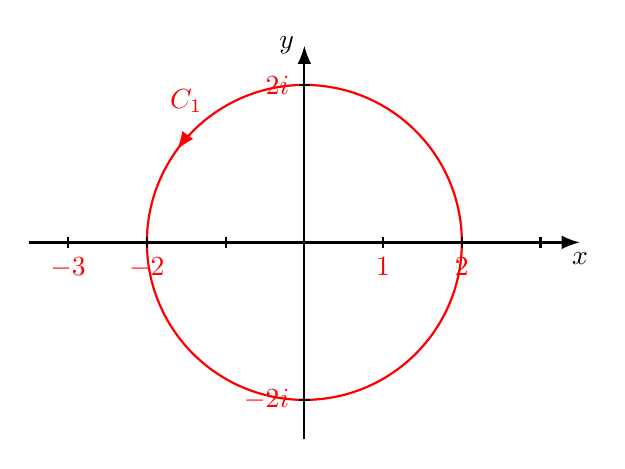
\begin{tikzpicture}[
    >=Latex, % Set default arrow tip style
    axis/.style={->, thick}, % Style for axes
    pathstyle/.style={red, thick}, % Style for the circle path
    labelstyle/.style={red}, % Style for labels
    tick/.style={thick}, % Style for tick marks
    % Style for placing a CCW arrow (<) on a path
    midarrowL/.style={
        decoration={markings, mark=at position 0.7 with {\arrowreversed{Latex}}},
        postaction={decorate}
    },
    midarrow/.style={
        decoration={markings, mark=at position 0.4 with {\arrow{Latex}}},
        postaction={decorate}
    }
]

    % Define radius
    \def\radius{2}

    % Axes (adjust limits to include ticks)
    \draw[axis] (-3.5, 0) -- (3.5, 0) node[below] {$x$};
    \draw[axis] (0, -2.5) -- (0, 2.5) node[left] {$y$};

    % Draw the red circle with counter-clockwise arrow
    \draw[pathstyle, midarrow, red] (0,0) circle (\radius); % Arrow at pos 0.375 (top-left)

    % Ticks and Labels on x-axis
    \foreach \x/\xlab in {-3/{-3}, -2/{-2}, -1/, 1/{1}, 2/{2}, 3/} { % Added tick at -1, 1, 3, removed label 3
        \draw[tick] (\x, -2pt) -- (\x, 2pt);
        \ifx\xlab\empty\else % Only add label if \xlab is not empty
            \node[labelstyle, below=2pt] at (\x, 0) {$\xlab$};
        \fi
    }

    % Ticks and Labels on y-axis
    % Use \ylab to store the label text
    \foreach \y/\ylab in {-2/{-2i}, 2/{2i}} {
        \draw[tick] (-2pt, \y) -- (2pt, \y);
        \node[labelstyle, left=2pt] at (0, \y) {$\ylab$};
    }

    % Label for the curve C1
    \node[labelstyle] at (-1.5, 1.8) {$C_1$}; % Position near the arrow

\end{tikzpicture}
\end{document}